%!TEX TS-program = ../make.zsh

\section{Experimental Background}
\label{sec:experimental_background}

\subsection{\icecube Detector}

The \icecube neutrino detector is built into a cubic-kilometer of the glacial ice at Earth's South Pole. 5160 photo detecting optical modules have been deployed between $1450\m$ and $2450\m$ below the surface. Construction has begun in 2005 with the deployment of the first optical modules. The detector is fully operational since 2010. \cite{instrumentation}

The optical modules are anchored on 86 vertical cables called \textit{strings}, which are positioned on a triangular grid with an overall hexagonal footprint. The strings are about $125\m$ apart. Each string holds 60 optical modules with a vertical spacing of $17\m$. \cite{instrumentation}

\begin{figure}[htbp]
  \smallerimage{icecube-schematics-instrumentation}
  \caption{Schematic overview of the \icecube detector. Image source: \cite{instrumentation}}
  \label{fig:aiThai0e}
\end{figure}

Additional to this \textit{in-ice array}, which is designed to measure neutrinos with energies from the TeV to the PeV scale, the \textit{DeepCore} sub array hold additional optical modules in order to lower the detection energy threshold in this region of the detector to detect neutrinos with energies from $10\GeV$ to $100\GeV$. \cite{instrumentation}


\subsection{Digital Optical Modules (DOMs)}
\label{sec:doms}

The basic detection unit in \icecube is the \textit{Digital Optical Module} (DOM). It consists of a glass sphere, a 10-inch photo multiplier tube (PMT), processing circuitry, and a flasher board with light-emitting diodes (LEDs) for calibration purposes (figure \ref{fig:aK4raigh}). \cite{instrumentation}

\begin{figure}[htbp]
  \subcaptionbox{The main components of the optical module are the photo multiplier tube (PMT), which detects impacting photons, the main electronics board that digitizes the signal and transmits the information to the surface, and the flasher board containing light-emitting diodes (LEDs) for calibration purposes. Image source: \cite{instrumentation}}{\halfimage{dom-components-instrumentation}}\hfill
  \subcaptionbox{The components of the module are contained within a glass sphere that can withstand high pressures. The space in between is filled with a gel to avoid optical effects at the medium boundaries. Image source: \cite{gallerynoharness}}{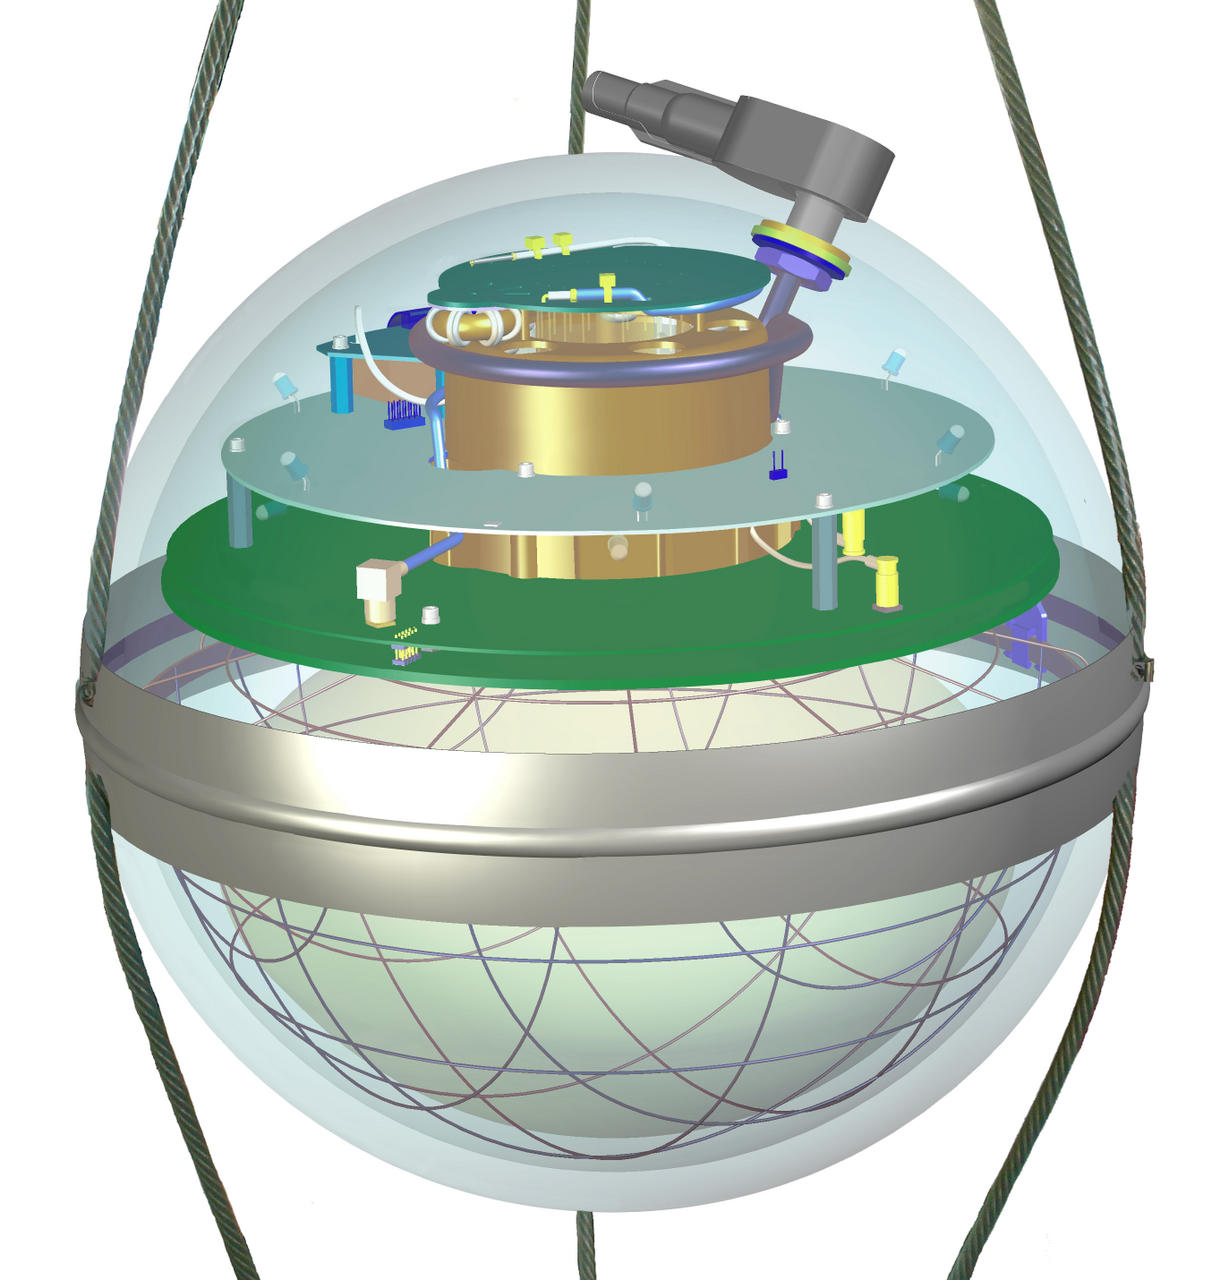
\includegraphics[width=0.35\textwidth]{img/DOMNoHarnessWhiteback_lg-gallery-2013}}
  \caption{Schematic display of a digital optical module (DOM), \icecube's basic detection unit. The module has an outer diameter of about $35\cm$. 5160 of these modules have been deployed in the glacial ice.}
  \label{fig:aK4raigh}
\end{figure}

% Other images:
% dom-8-top-hemisphere-and-penetrator-gallery-2011, source: Megan Madsen, 2011, https://gallery.icecube.wisc.edu/internal/v/GraphicRe/graphics/dom/8-top-hemisphere-and-penetrator.png.html
% dom-schematics-firstyearperformance, source: \cite{firstyearperformance}

The recorded signals from the PMT are digitized within the module before sending the signal to the surface in order to minimize the loss of information from degradation of analog signals sent over long distances. \cite{firstyearperformance}

The optical modules are optimized for detecting Cherenkov light emitted by particles with energies from $10\GeV$ to $10\PeV$ up to $500\m$ away from the optical module. \cite{instrumentation}


\subsection{Properties of South-Polar Ice}
\label{sec:ice}

#### intro, method
- antarctic ice has exceptional optical properties because air bubbles shrink and vanish under large pressure forming an air clathrate hydrate \cite{rongenswedishcamera}
- using the LED flasher calibration system,
- properties of the glacial ice of \icecube have been measured
- average distance to absorption $\lambda\abs$
- average distance between successive scatters $\lambda\sca$
- angular distribution of the new direction \cite{icepaper}
- ice in layers of arbitrary thickness of $10\m$
- fit the parameters within these layers such that the properites are best interpreted as average of their true values over the thickness of the layers \cite{icepaper}


#### scattering
The South-Polar ice has shown to be preferentially forward scattering with a mean cosine of the scattering angle of $\meancostheta = 0.94$ with only a weak dependence on the wavelength. \cite{ackermann}
% ackermann, paragraph 9

% Typical scattering length:
% average esca = 25m \cite{lundberg}
% scattering lengths between 5m and 90m in the detector volume \cite{ppcpaper}
% effective scattering coefficient for 400nm between 0.011/m and 0.2/m \cite{icepaper} fig. 16, corresponding to esca=5m to 90m esca

Typical effective scattering lengths within the South-Polar ice are in the order of $25\m$ \cite{lundberg} and range from $5\m$ to $90\m$ in the detector volume \cite{icepaper}, corresponding to the geometric scattering length ranging from $0.3\m$ to $5.4\m$.

- air bubble do not cause absorption, only scattering \cite{absorption1997}
- effective scattering coefficient $b_\text{e} := \sfrac{1}{\lambda\esca}$
- wave-length dependence from theoretical models of light scattering in dusty ice and AMANDA measurements, $b_\text{e} = b_\text{e}(\nu = 400\nm) \cdot \left(\frac{\nu}{400\nm}\right)^{-\alpha}$, $\alpha$ global fit parameter

\begin{figure}[htbp]
  \subcaptionbox{}{\halfimage{icepaper-fig-16-esca}}\hfill
  \subcaptionbox{}{\halfimage{icepaper-fig-16-abs}}
  \caption{Values of the absorption length $\lambda\abs$ and the effective scattering length $\lambda\esca$ for different depths. Plot taken from \cite[figure 16]{icepaper}. A detailled data table is given in \cite[table C1]{icepaper}.}
  \label{fig:Ahxobai3}
\end{figure}

#### absorption
- Absorption lengths in the South-Polar ice vary between $20\m$ in dusty regions and $280\m$ in very clear ice layers. \cite{ackermann, ppcpaper, icepaper}
- absorption coefficient $a := \sfrac{1}{\lambda\abs}$
- for absorption: $a(\nu) = a_\text{dust}(\nu) + A \e^{-B/\nu} (1 + 0.01 \delta\tau)$, $a_\text{dust}(\nu) = a_\text{dust}(\nu = 400\nm) \left(\frac{\nu}{400\nm}\right)^{-\kappa}$, $\delta\tau(d) = T(d) - T(1730\m)$ for depth $d$
- layer of ice containing the most dust at around $2000\m$ (``dust peak'')

#### tilt
- following the layers of dust concentration, ice layers also with tilt

\begin{figure}[htbp]
  \centering
  \smallerimage{icepaper-fig-14-layers}
  \caption{Ice layers along the average gradient direction within the ice. The relief is amplified by a factor of 3 to enhance the clarity of the layer structure. The lowest layer shown exhibits a shift of $56\m$ betweeen its shallowest and deepest points, which is the largest shift of all layers shown in the figure. Plot and caption taken from \cite[figure 14]{icepaper}.}
  \label{fig:wohr8uaY}
\end{figure}

#### anisotropy
- anisotropic scattering amplitude, aligned with ice flow direction \cite{icrc17pocam}


#### ice models
- timeline of ice models: \url{https://docushare.icecube.wisc.edu/dsweb/Get/Document-79091/ice.pdf} \cite{flasherdataderivedicemodels}





\subsection{Hole Ice Around the Detector Strings}
\label{sec:hole_ice}

\begin{figure}[htbp]
  \smallerimage{swedish-camera-downwards}
  \caption{Image source: \cite{icrc17pocam}}
  \label{fig:label}
\end{figure}

- The hole ice is refrozen water. When the bulk ice within the drill hole became water the structures that were responsible for the specific properties of that bulk-ice layer were destroyed. The refreezing happens the same way everywhere in the drill hole.

- camera suggests two hole-ice components: clear outer region, central column of small scattering length about 16cm diameter \cite{rongenswedishcamera,instrumentation}
- cylindrical freezing: impurities or air bubbles are pushed along the freezing boundaries until they merge in the center \cite{rongenswedishcamera}

- 68 boreholes, approx 60cm diameter to depth of 250m using hot water drilling\cite{instrumentation}
- instrumentation deployed into the water-filled holes, becoming frozen in place and optically coupled with the surrounding sheet \cite{instrumentation}
- produce hole 48h, freezing about 2weeks \cite{instrumentation}

- camera deployed to monitor the freeze-in process and optical properties of drill hole. Two video cameras in separate spheres, each also equipped with four LEDs and three lasers. \cite{instrumentation}
- drill hole completely refrozen after 15 days \cite{instrumentation}
- clear outer layer and central core of about 16cm diameter with smaller scattering length than bulk ice\cite{instrumentation}
- no long-term changes have been observed \cite{instrumentation}

